% easychair.tex,v 3.5 2017/03/15

\documentclass{easychair}
%\documentclass[EPiC]{easychair}
%\documentclass[EPiCempty]{easychair}
%\documentclass[debug]{easychair}
%\documentclass[verbose]{easychair}
%\documentclass[notimes]{easychair}
%\documentclass[withtimes]{easychair}
%\documentclass[a4paper]{easychair}
%\documentclass[letterpaper]{easychair}

\usepackage{doc}
\usepackage{amssymb}


%%%%%%%%%%%%%%%%%%%%%%%%%%%
\usepackage{fancyhdr} % Custom headers and footers
\pagestyle{fancyplain} % Makes all pages in the document conform to the custom headers and footers
\fancyfoot[C]{\thepage}% Page numbering for center footer 
\fancyfoot[L]{}% nothing in left footer
\fancyfoot[R]{}% nothing in right footer
%%%%%%%%%%%%%%%%%%%%%%%%%%%

% use this if you have a long article and want to create an index
% \usepackage{makeidx}

% In order to save space or manage large tables or figures in a
% landcape-like text, you can use the rotating and pdflscape
% packages. Uncomment the desired from the below.
%
% \usepackage{rotating}
% \usepackage{pdflscape}

% Some of our commands for this guide.
%
%\newcommand{\easychair}{\textsf{easychair}}
%\newcommand{\miktex}{MiK{\TeX}}
%\newcommand{\texniccenter}{{\TeX}nicCenter}
%\newcommand{\makefile}{\texttt{Makefile}}
%\newcommand{\latexeditor}{LEd}

%\makeindex

%% Front Matter
%%
% Regular title as in the article class.
%
\title{Random Walks with Memory Applied to Grand Slam Tennis Matches Modeling}

% Authors are joined by \and. Their affiliations are given by \inst, which indexes
% into the list defined using \institute
%
\author{Tomáš Kouřim}

% Institutes for affiliations are also joined by \and,
\institute{
  Institute of Information Theory and Automation, Czech Academy of Sciences
  Prague, Czech Republic\\
  \email{kourim@outlook.com}
 }

%  \authorrunning{} has to be set for the shorter version of the authors' names;
% otherwise a warning will be rendered in the running heads. When processed by
% EasyChair, this command is mandatory: a document without \authorrunning
% will be rejected by EasyChair

\authorrunning{Tomáš Kouřim}

% \titlerunning{} has to be set to either the main title or its shorter
% version for the running heads. When processed by
% EasyChair, this command is mandatory: a document without \titlerunning
% will be rejected by EasyChair
\titlerunning{Random Walks in Tennis Modeling}
\begin{document}
\maketitle
\begin{abstract}
The contribution presents a model of a random walk with varying transition
probabilities implicitly depending on the entire history of the walk,
which is an improvement of a model with varying step sizes. The transition
probabilities are altered according to the last step of the walker
using a memory parameter to either reward or punish success by increasing
or decreasing its probability in the next step. This walk is applied
to model Grand Slam tennis matches and fitted on their entire history
since 2009. The suitability of the model is thoroughly tested on a
number of real datasets. The model seems to be robust and describe
well the majority of matches, making it an useful tool to produce
precise \emph{in-play} odds.
\end{abstract}

%\setcounter{tocdepth}{2}
%{\small
%\tableofcontents}


\section{Introduction}

Tennis is one of the most popular sports both on professional and
amateur level. Millions of people pursue tennis as their leisure time
activity \cite{pac2019report} and same numbers hold also for the
people following and watching the professional tennis competitions.
Tennis also plays a major role in the sports betting industry, which
grows rapidly and becomes more and more important part of the global
economy. In the Czech Republic only, the total sales in sports betting
industry reached CZK 64.5 billion (2.9 billion USD) in 2017, representing
$1.3\%$ of Czech GDP \cite{mf2017report}. The immense size of the
betting market attracts also many fraudsters. The European Sports
Security Association regularly reports on suspicious betting activities,
the latest report (2018) contained 267 cases of such activity, 178
(67\%) in tennis \cite{essa2018fullreport}. It is thus obvious that
a precise model describing the game of tennis has many possible uses
in real life.

Tennis is also a sport more than suitable to be modeled using random
walks or random processes in general, as it naturally consists of
many such processes. A series of tennis matches is a random walk,
the sequence of sets within a match, games within a set, points within
a game or even strokes within a point can be all considered a random
process and modeled using a random walk. Additionally, these walks
are well described by the tennis rules and there exist lots of data
describing these random processes (i.e. various tennis result databases
provided by the tennis federation as well as many private subjects).
In this paper, the random walk consisting of a sequence of sets within
a match is studied. Matches played as a \emph{best-of-five}, i.e.
the men Grand Slam tournaments, are considered in this paper. In these
matches, up to 5 steps of the random walk can be observed, making
them more suitable than the \emph{best-of-three }games, where maximum
3 steps can occur.

The matches are modeled using a new type of a recently introduced
random walk with varying probabilities \cite{ja2017ddny}, which is
a modification of a random walk with varying step size introduced
by Turban \cite{turban2010random}. It seems more than suitable to
model tennis matches as the data suggest that a success in tennis
yields another success, or in other words, that winning one particular
part of the match increases the chances of winning the next part as
well. This behavior is well described by the new random walk model.

The paper is organized as follows. Next chapter introduces the new
type of random walk used for tennis modeling. Section \ref{sec:Data-description}
provides general description of the data used, Section \ref{sec:Initial-probability-derivation}
shows how to obtain starting probabilities. In Chapter \ref{sec:Model-description-and}
the actual model is described and its performance is evaluated. Section
\ref{sec:Conclusion} concludes this paper.

\section{Random walk with varying probability\label{sec:Random-walk-with}}

In 2010, Turban described \cite{turban2010random} a new version of
a random walk with memory, where the memory is introduced using variable
step size. This idea was further extended by Kouřim \cite{ja2017ddny,ja2019teze}
and an alternative version of a random walk with memory was introduced,
where the memory affects the walk through varying transition probabilities.

The walk evolves in a following way. Initial step is made following
the result of a Bernoulli random variable with starting probability
parameter $p_{0}$, that is, 
\[
P(X_{1}=``right")=p_{0}.
\]
 From the second step on, the transition probability in the $t-th$
step is given by 
\[
X_{t-1}=``right"\Longrightarrow P(X_{t}=``right")=\lambda p_{t-1}
\]

\[
X_{t-1}=``left"\Longrightarrow P(X_{t}=``right")=1-\lambda(1-p_{t-1})
\]
 for some $\lambda\in(0,\,1).$ When the directions are formalized
so that $``right"\approx1$ and $``left"\approx-1$, the formula for
the $t-th$ transition probability can be rewritten as
\begin{equation}
p_{t}=\lambda p_{t-1}+\frac{1}{2}(1-\lambda)(1-X_{t}).\label{eq:suc_punished}
\end{equation}

This definition of a random walk means that the opposite direction
is always preferred and that the walk tends to return back to the
origin. Alternatively, inverse approach can be applied and the same
decision can be supported. Formally, the expression for the $t-th$
transition probability is then 
\begin{equation}
p_{t}=\lambda p_{t-1}+\frac{1}{2}(1-\lambda)(1+X_{t}).\label{eq:suc_rew}
\end{equation}

For more details on the walk and its rigorous definition, see the
original papers \cite{ja2017ddny,ja2019teze}.

\section{Data description\label{sec:Data-description}}

For the purpose of this study, a database containing the results from
all Grand Slam tournaments from 2009 to 2018 and corresponding Pinnacle
Sports bookmaker's odds\footnote{This bookmaker is considered leading in the sports betting industry.}
was created based on the information publicly available from website
www.oddsportal.com. There are 4 Grand Slam\footnote{Australian Open, French Open, The Wimbledon and US Open.}
tournaments each year, 40 tournaments together. Each Grand Slam has
$128$ participants playing in a single-elimination system (i.e. $127$
games per tournament), making it a set of $5080$ games together.
However, the games where either one of the players retired were omitted
from the dataset and so were the matches where no bookmaker's odds
were available. Together there were $4255$ matches with complete
data available, presenting total $432$ players. The most active player
was Novak Djokovic, who participated in 188 matches. On average, each
player played 19.7 matches, with the median value of 8 matches played.
The most common result was 3:0, occurring 2138 times, on the other
hand, 5 sets were played only 808 times.

The order in which the players are listed is rather random. The first
listed players\footnote{Such player/team would be normally considered as ``home'', however,
as there are (usually) no home players on the international tournaments,
the order is based on the www.oddsportal.com data and/or the respective
tournament committees.} won 2201 in total, just slightly over the half. On the other hand,
if the bookmaker's favorite (i.e. the player with better odds or the
first listed player in case the odds are even) is considered, the
situation changes significantly. The favorites won 3307 matches in
total, mostly 3:0, and lost 311 times 0:3, 347 times 1:3 and 290 times
2:3. It suggests that bookmaker's odds can be used as a probability
estimate, which is in accordance with previous results, for example
\cite{ja2016ddny}.

\section{Initial probability derivation\label{sec:Initial-probability-derivation}}

The model of a random walk with varying probabilities described in
Section \ref{sec:Random-walk-with} takes two parameters, initial
set winning probability $p_{0}$ and the memory coefficient $\lambda$.
Finding the optimal value of $\lambda$ is the main subject of this
paper and is described in Section \ref{sec:Model-description-and}.

Estimating the initial set winning probability is a major task by
itself and represents one of the elementary problems in tennis modeling.
For the purpose of this article an estimation based on bookmaker's
odds will be used. Specifically, the closing odds\footnote{Closing odds means the last odds available before the match started.}
by Pinnacle Sports bookmaker for the first set result are used to
estimate the probabilities of each player winning the first set, i.e.
$p_{0}$ and $1-p_{0}$. Such odds represent a good estimation of
the underlying winning probability and are considered as a baseline
in the sports betting industry. The odds, however, have to be transformed
into probabilities. A method described in \cite{ja2015ddny} is used
to obtain probabilities, using a parameter $t\in[0,\,1]$ set to the
value $t=0.5$. Obtained first set winning probabilities are then
used as a given starting probability $p_{0}$ in the random walk.

\section{Model description and evaluation\label{sec:Model-description-and}}

\subsection{Model description}

Original inspiration of the random walk described in Section \ref{sec:Random-walk-with}
is based on intensive study of historical sport results and their
development. The data suggest that the probability of success (i.e.
scoring, winning a set or a point etc.) evolves according to the random
walk with varying probabilities. Moreover, it follows from the data
that sports can be very roughly divided into two categories. Sports
played for a certain amount of time, such as soccer or ice-hockey,
evolve according to the walk defined by expression \ref{eq:suc_punished}.
On the other hand, sports where there is necessary to achieve certain
number of points, such as tennis or volleyball, appear to follow the
pattern defined in equation \ref{eq:suc_rew}. Therefore the later
approach is used to model a tennis game.

The model is used to predict the winning probabilities of sets 2 through
5 and is constructed in a following manner. For each match, the first
set winning probability of Player A\footnote{The player which is listed first in the database, see Section \ref{sec:Data-description}
for details.}, $p_{0}$, is given (see Section \ref{sec:Initial-probability-derivation})
and a coefficient $\lambda$ is fixed for the entire dataset. In order
to compute the second set winning probability\footnote{Winning probability of Player A is always considered as Player B winning
probability is just the complement.}, the result of the first set is observed and second set winning probability
is computed using equation \ref{eq:suc_rew}. This procedure is repeated
for all remaining sets played.\footnote{There can be either 3, 4 or 5 sets played in total in a \emph{best-of-five}
tennis game.}

\subsection{Model evaluation}

In order to verify the model's accuracy, several tests were performed.
First, the dataset was divided into training and testing sets. The
division can be done naturally by the order of games played. Given
a specific time, past matches constitute to a training set, future
matches to a testing set. For the purpose of this paper, the split
was done on a yearly basis, the data from one previous tennis season
were used as a training set to predict winning probabilities in the
following season, considered the testing set (i.e. 2010 was the first
season used as testing data, 2017 was the last season used as training
data), making it 9 training/testing splits together. Another approach
to dataset splitting is to consider data from all previous years as
testing data and from one future year as training data, however, previous
study shows that the difference between these two approaches is negligible
\cite{ja2016ddny}.

Next step in model verification is the estimation of parameter $\lambda$.
Training sets and maximal-likelihood estimates were used for this
task. The likelihood function is defined as 
\[
L=\prod_{i=1}^{N_{train}}(x_{i}p_{i}+(1-x_{i})(1-p_{i})),
\]
where $N_{train}$ is the number of sets 2 thru 5 played in the training
dataset, $p_{i}$ is Player A's winning probability in the $i-th$
set obtained using equation \ref{sec:Random-walk-with} for each match,
and $x_{i}$ is the result of the $i-th$ set, $x_{i}=1$ if Player
A won the $i-th$ set, $x_{i}=0$ otherwise. For computational reasons
the \emph{log-likelihood }$L_{l}=log(L)$ was used, i.e. the function
\[
L_{l}=\sum_{i=1}^{N_{train}}log(x_{i}p_{i}+(1-x_{i})(1-p_{i}))
\]
was maximized. Numerical methods implemented in Python library SciPy
were used to obtain specific values of $\lambda$. The optimal values
of the coefficient $\lambda$ can be seen in Table \ref{tab:Optimal-values-of}.

\begin{table}
\begin{centering}
\begin{tabular}{|c|c|}
\hline 
Year & Optimal lambda\tabularnewline
\hline 
\hline 
2010 & 0.8074\tabularnewline
\hline 
2011 & 0.8497\tabularnewline
\hline 
2012 & 0.8142\tabularnewline
\hline 
2013 & 0.9162\tabularnewline
\hline 
2014 & 0.8523\tabularnewline
\hline 
2015 & 0.8429\tabularnewline
\hline 
2016 & 0.8920\tabularnewline
\hline 
2017 & 0.8674\tabularnewline
\hline 
2018 & 0.8333\tabularnewline
\hline 
\end{tabular}
\par\end{centering}
\caption{\label{tab:Optimal-values-of}Optimal values of the coefficient $\lambda$
for respective years.}

\end{table}

Finally, the model was used to predict set winning probabilities of
the unseen data from the training set using initial bookmaker derived
odds, equation \ref{eq:suc_rew} and memory parameter $\lambda$ obtained
from the corresponding training set. In order to verify the quality
of the model, the average theoretical set winning probability of Player
A $\hat{p}=\frac{1}{n}\sum_{i=1}^{N_{test}}p_{i}$ and its variance
$\hat{\sigma}^{2}=\frac{1}{n}\sum_{i=1}^{N_{test}}p_{i}(1-p_{i})$
were computed and so was the observed Player A winning ratio $\bar{x}=\frac{1}{n}\sum_{i=1}^{N_{test}}x_{i}$.
Using the Lyapunov variant of Central Limit Theorem \cite{billingsley1995probability},
the resulting random variable $y$ follows the standard normal distribution
\[
y=\frac{\sqrt{N_{test}}(\bar{x}-\hat{p})}{\hat{\sigma}}\thicksim\mathcal{N}(0,\,1).
\]
Then ow to verify the model accuracy, the the null hypothesis that
the true average Player A set winning probability $\bar{p}$ equals
$\hat{p}$ against the alternative hypothesis $\bar{p}\neq\hat{p}$
was tested. Formally, 
\[
H_{0}:\bar{p}=\hat{p}
\]
\[
H_{1}:\bar{p}\neq\hat{p}.
\]

One of the assumptions of the CLT is that the observed random variables
are independent. This is obviously not true in the case when $N_{test}$
contains all sets from the testing data. Quite the opposite, the model
assumes that the winning probability of a set directly depends on
the winning probability of the previous set. This can be easily solved
by splitting the testing dataset into 4 subsets containing only results
from single set of each match, i.e. sets 2, 3, 4 and 5 (if they were
played). The matches can be considered independent from each other
and so can be the $i-th$ sets of respective matches.

Using this approach, there are 36 testing sets\footnote{Up to 4 sets considered in each match, 9 yearly testing datasets.}
together. On a 95\% confidence level, only on 2 out of the 36 available
subsets provide strong enough evidence to reject the null hypothesis.
On the other hand, the null hypothesis is relatively weak. It only
says that the prediction is correct on average. In order to verify
the quality of the predictions, more detailed tests have to be created.
This can be done primarily by testing the null hypothesis on many
subsets created according to some real life based criteria. The natural
way how to create such subsets is dividing the matches to the 4 different
tournaments. This refining yields 180 subsets\footnote{4 sets in each match evaluated, 4+1 tournaments every year, 9 years
for testing.} altogether. Using 95\% confidence level, only 6 of the 180 subsets
have data strong enough to reject the null hypothesis. It is worth
mentioning that the size of some of the datasets regarding fifth sets
is only slightly above 20 observations, which can interfere with the
assumptions justifying the use of Central Limit Theorem.

To further analyze the robustness of the model it is important to
realize the structure of the data. So far, the player, whose winning
probability was estimated, was chosen arbitrarily based on some external
(more or less random) order. As such, the observed winning probability
in every subset equals approximately to $\frac{1}{2}$, see further
Section \ref{sec:Data-description}. In such a dataset it is not very
difficult to estimate the average winning probability. The situation
changes if the bookmaker's favorite is considered for predictions
(more details on who is the favorite and how to choose him in Section
\ref{sec:Data-description}). Performing the same tests as described
in the previous paragraph the data allows to reject the null hypothesis
(at 95\% confidence level) on 5 subsets containing all tournaments
and 8 single tournament subsets (out of 180 subsets total).

Finally, the testing data can be divided into groups using the initial
probability $p_{0}$. Such a division is based on an assumption that
the matches with similar bookmaker odds should have similar development.
The matches are divided into 5 groups, each containing 10 percentage
points in first set winning probability. Except for the biggest favorites
(with first set winning probability over 90\%), this division seems
reasonable. The data histogram can be seen on Figure \ref{fig:First-set-winning}.
Out of the 180\footnote{Further division, i.e. by tournament and odds, was not performed as
the resulting datasets would not contain enough data.} newly created odds-based subgroups, only 9 have data strong enough
to reject $H_{0}$ on a 95\% confidence level. The entire results
of the hypothesis testing (the \emph{p-values }of respective tests)
can be seen on Figure \ref{fig:p-values-of-hypothesis}.

\begin{figure}

\begin{centering}
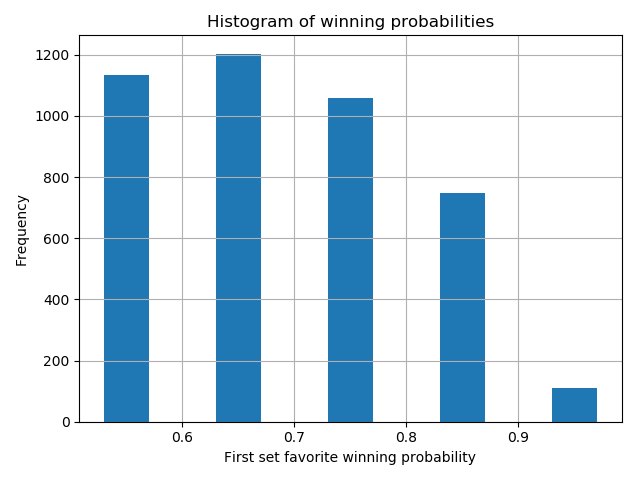
\includegraphics[width=1\textwidth]{probabilities_histogram}\caption{\label{fig:First-set-winning}First set winning probability $p_{0}$
histogram.}
\par\end{centering}
\end{figure}

\begin{figure}
\begin{centering}
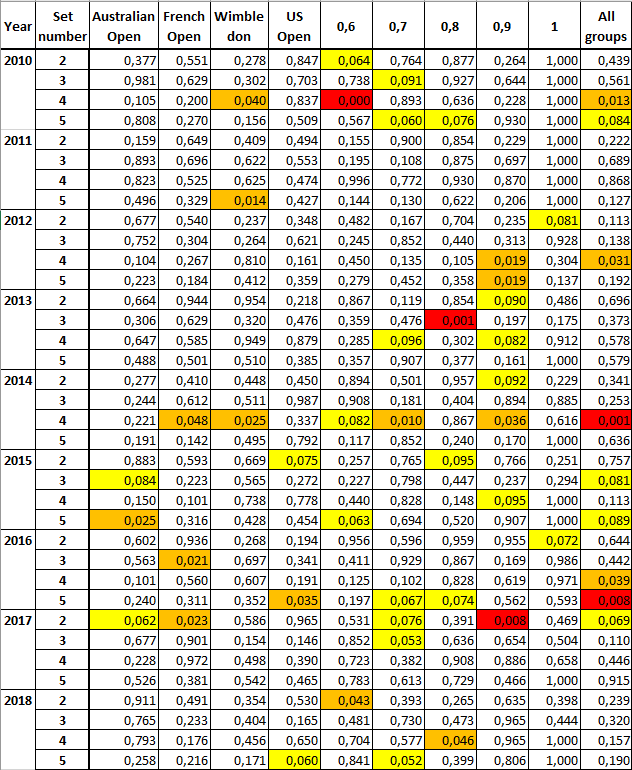
\includegraphics[width=1\textwidth]{hypothesis_testing.PNG}\caption{\emph{\label{fig:p-values-of-hypothesis}p-values} of hypothesis tests
for different testing sets. Red are marked those allowing to reject
$H_{0}$ on 99\% confidence level, orange on 95\% and yellow on 90\%
confidence level.}
\par\end{centering}
\centering{}
\end{figure}

Overall, the model was tested on 360 different subsets and only 22
of them (6.1\%) provided enough evidence to reject $H_{0}$ on 95\%
confidence level. These subsets are distributed randomly and there
is no pattern among them, indicating there is no systematic bias in
the model. The random walk with varying probabilities thus seems to
be a robust model which can be used to precisely predict set winning
probabilities in men tennis Grand Slam matches.

\section{Conclusion\label{sec:Conclusion}}

This paper describes the random walk with varying probabilities and
its application on Grand Slam tennis data. A model describing the
development of a single match is introduced and tested on a dataset
containing all matches from seasons 2009-2018. The results show that
the model is robust and performs well on the absolute majority of
reasonable data subsets. This suggest that the model could be used
as a tool to generate precise \emph{in-play} odds during the matches
or to directly compete against the odds currently provided by the
bookmakers.

\section{Remarks}

The source code containing all functionality mentioned in this article
is freely available as open source at GitHub\footnote{https://github.com/tomaskourim/mathsport2019}
together with a database containing all data that was used in this
paper. Some results can be also obtained from the same repository.

\bibliographystyle{plain}
\bibliography{doktknih}

\end{document}
